\documentclass[xcolor=table,9pt]{beamer}

\usetheme{Frankfurt}
\usecolortheme{crane}
\useinnertheme{circles}

\usepackage{color, colortbl}
\usepackage{amsmath}
\usepackage{graphicx}
\usepackage{float}
\usepackage{wrapfig}
\usepackage{multicol}
\usepackage{dcolumn,array}
\usepackage{booktabs}
\usepackage{geometry}
\usepackage{caption}
\usepackage{subcaption}
\usepackage{bbm}
\usepackage{bm}
\usepackage{natbib}
\usepackage{stackengine} 
\usepackage{multirow}

\definecolor{Gray}{gray}{0.8}

\stackMath


\begin{document}
\title{Three Essays on Shrinkage Estimation and Model Selection of Linear and Nonlinear Time Series Models}   
\author{Mario Giacomazzo } 
\date{9 May 2018} 

\frame{\titlepage} 





%%%%%%%%%%%%%%%%%%%%%%%%%%%%%%%%%%%%%%%%%%%%%%%%%%%%%%%%%%%%%%%%%%%%%%%%
%% START: INTRODUCTION
%%%%%%%%%%%%%%%%%%%%%%%%%%%%%%%%%%%%%%%%%%%%%%%%%%%%%%%%%%%%%%%%%%%%%%%%
\frame{\frametitle{Overview and Motivation} 
\begin{itemize}
\item Parametric Time Series Models \\~\
\begin{itemize}
 \item Logistic Smooth Transition Autoregressive Model (LSTAR) \citep{Terasvirta1994}
 \item Threshold Autoregressive Model (TAR)  \citep{Tong1990}
 \item Autoregressive Moving Average Model (ARMA)  \citep{Box1970} \\~\
\end{itemize}
\item Model Differences \\~\
\begin{itemize}
	\item ARMA = Popularized for Weakly Stationary Time Series
	\item LSTAR and TAR = Handling Nonlinear Behavior
	\begin{itemize}
		\item Changes in Level, Dynamics, and Volatility
		\item Alternative Approach to Handling Nonstationary and Cyclical Phenomenon
		\item Useful for Clustering and Classification of Realizations
	\end{itemize}
\end{itemize}
\end{itemize}
}

\frame{\frametitle{Overview and Motivation} 
\begin{itemize}
\item Purpose \\~\
\begin{itemize}
\item Primary Goal is Forecasting
\item Economic Variables: Past Realizations Assist in Prediction \citep{Mann1943}
\item Estimation and Fitting of ARMA \citep{Durbin1960}
\item Practical Procedures Developed for Industrial Engineering \citep{Box1970}
\item Asymmetries Noticed in US Unemployment \citep{Rothman1988,Montgomery1998,Koop1999}
\end{itemize}
\end{itemize}
}

\frame{\frametitle{Overview and Motivation} 
\begin{itemize}
	\item Model Complexity \\~\
	\begin{itemize}
		\item Determined by Order Parameters
		\begin{itemize}
			\item Autoregressive (AR)
			\item Moving Average (MA)
			\item Distributed Lag (DL)
			\item Regime-specific Model Orders \\~\
		\end{itemize}
		\item Frequentist Approach: Select Based on Information Criteria or Forecasting Performance \\~\
		\item Bayesian Approach: Reversible jump Markov Chain Monte Carlo (RJMCMC) \citep{Green1995}
		\begin{itemize}
			\item AR(P) \citep{Troughton1997}
			\item TAR(P) \citep{Campbell2004,Nieto2013}
			\item STAR(P) \citep{Lopes2006}
		\end{itemize}
	\end{itemize}
\end{itemize}
}

\frame{\frametitle{Overview and Motivation} 
\begin{itemize}
	\item Model Complexity (Cont.) \\~\
	\begin{itemize}
		\item Problem
		\begin{itemize} 
			\item Difficult When Multiple Order Parameters Must Be Chosen
			\item Often Leads to Inflexible Representations
			\item Overfitting Can Still Occur \\~\
		\end{itemize}
		\item Solution 
		\begin{itemize}
			\item Intentionally Fix Orders to Be Large
			\item Restructure Time Series Model as a High Dimensional Linear Regression
			\item Apply Penalized Estimation Methods Aimed at Sparse Models
		\end{itemize}
	\end{itemize}
\end{itemize}
}

\frame{\frametitle{Introduction: Overview and Motivation} 
	\begin{center}
	\Huge \underline{Dissertation Theme} \\
	
	\huge Bayesian Automatic Estimation and Variable Selection Procedures for Flexible Subset Models
	\end{center}
}









%%%%%%%%%%%%%%%%%%%%%%%%%%%%%%%%%%%%%%%%%%%%%%%%%%%%%%%%%%%%%%%%%%%%%%%%
%% CHAPTER 2: LOGISTIC SMOOTH TRANSITION AUTOREGRESSIVE MODEL
%%%%%%%%%%%%%%%%%%%%%%%%%%%%%%%%%%%%%%%%%%%%%%%%%%%%%%%%%%%%%%%%%%%%%%%%
\frame{\frametitle{Chapter 1: LSTAR Model} 

\begin{itemize}
\item Gaussian LSTAR$(P)$ Model With 2-Regimes \\~\
\begin{itemize}
\item Given autoregressive order $P$, let $\bm{x}_t'=[y_{t-1},y_{t-2},\cdots,y_{t-P}]$, $\bm{\alpha}'=[\alpha_1,\cdots,\alpha_P]$, and $\bm{\beta}'=[\beta_1,\cdots,\beta_P]$. 

$$y_t=(\mu_\alpha+\bm{x}'_t\bm{\alpha})(1-G(z_{t}))+(\mu_\beta+\bm{x}'_{t}\bm{\beta}+)G(z_{t})+\epsilon_t$$

where $\epsilon_{t}\sim \textrm{ i.i.d. } N(0,\sigma^2)$ and $G(z_t): \mathbb{R}\to\mathbbm{G}\subseteq[0,1]$. \\~\

\item For LSTAR, consider transition function $G(\cdot)$ such that
$$G(z_t,\gamma^*,\delta)=\{1+\exp[-(\gamma^*/s_Z)(z_t-\delta)]\}^{-1}$$
\begin{itemize}
	\item Threshold Parameter $\delta$ Determines When Transition Occurs
	\item Slope Parameter $\gamma=\gamma^*/s_Z$ Determines the Rate of Transition
	\item As $\gamma \to \infty$, $G(z_t,\gamma^*,\delta)$ Becomes a Step Function
\end{itemize}
\end{itemize}
\end{itemize}
}

\frame{\frametitle{Chapter 1: LSTAR Model} 
\begin{itemize}
\item Prior Distributions\\~\
	\begin{itemize}
		\item TAR\citep{Geweke1993,Chen1995,Koop1999}, STAR\citep{Lubrano2000,Lopes2006,Livingston2017} \\~\
		\item $\mu_\alpha\sim \mathcal{N}(\cdot,\cdot)$ and $\mu_\beta\sim \mathcal{N}(\cdot,\cdot)$		
		\item $\sigma^2\sim\mathcal{IG}(\cdot,\cdot)$
		\item $\gamma^*\sim\mathcal{LN}(\cdot,\cdot)$
		\item  $\delta \sim \textrm{U}[q_Z(0.15),q_Z(0.85)]$ where $q_Z(\cdot)$ is the empirical quantile function
		\item Bayesian Global-Local Shrinkage Priors for $\bm{\alpha}$ and $\bm{\beta}$ 
				$$\alpha_k,\beta_k|\lambda^2_k,\lambda^2,\sigma^2 \sim N(0,\sigma^2\lambda^2\lambda^2_k)$$
		$$\lambda^2_k \sim \pi_{Local}(.) \textrm{ and  } \lambda^2 \sim \pi_{Global}(.)$$
	\begin{itemize}
		\item LASSO \citep{Park2008,Hans2009,Schmidt2013}
		\item Regime-Specific LASSO (Separate Global Tuning Parameters)
		\item Variable Selection LASSO \citep{Lykou2013}
		\item Horseshoe \citep{Carvalho2010,Makalic2016b}
	\end{itemize}
	\end{itemize}
\end{itemize}
}


\frame{\frametitle{Chapter 1: LSTAR Model} 
\begin{itemize}
\item Transition Variable\\~\
\begin{itemize}
\item Change-Point Option: $z_t=t$
\item Exogenous Option: $z_t=x_{t-d}$
\item Endogenous Option: $z_t=y_{t-d}$ (Self-Exciting)
\item Let $\bm{d}'_t=[y_{t-1},y_{t-2},\cdots,y_{t-d_{max}}]$ and $\bm{\phi}'_t=[\phi_{1},\phi_{2},\cdots,\phi_{d_{max}}]$. Reparameterize transition variable $z_t=\bm{\phi}'\bm{d}_t$. 

$$\bm{\phi}\sim Dir\bigg(\bigg[\frac{1}{d_{max}},\frac{1}{d_{max}},\cdots,\frac{1}{d_{max}}\bigg]'\bigg)$$

Now, $z_t$ is a weighted average of all considered transition variables. Because the weights are constrained to sum to $1$, the prior for $\delta$ does not require modification. \\~\

\item Advantages
\begin{itemize}
	\item Allows for a composite transition variable
	\item Estimates a more encompassing LSTAR model.
\end{itemize}
\end{itemize}
\end{itemize}
}

\frame{\frametitle{Chapter 1: LSTAR Model} 
\begin{itemize}
\item Simulation Study\\~\

 Let $\bm{d}_t=[y_{t-1},y_{t-2},y_{t-3},y_{t-4}]'$ and $\bm{\phi}'=[\phi_1,\phi_2,\phi_3,\phi_4]$. 
\begin{equation*}
	\begin{split}
		y_t&=(-0.6y_{t-3})[1-G(y_{t-1})]+(0.02+0.75y_{t-3})[G(y_{t-1})]+\epsilon_t\\
		& \textrm{where: } G(y_{t-1})=\bigg\{1+\exp\big[-120(\bm{\phi}'\bm{d}_t-0.02)\big]\bigg\}^{-1} \\
		&\textrm{ and }\epsilon_t \sim \textrm{i.i.d. }  N (0,0.02^2)\\
	\end{split}
\end{equation*}
Under  prior $\bm{\phi}\sim Dir([0.25,0.25,0.25,0.25]')$, we conduct posterior sampling for three different threshold variables $\{z_{1,t},z_{2,t},z_{3,t}\}$ defined through $\bm{\phi}$. BHS priors are used for autoregressive coefficients.
\end{itemize}
}

\frame{\frametitle{Chapter 1: LSTAR Model} 
\begin{figure}
	\centering
	\caption{Ten Random Replications}
	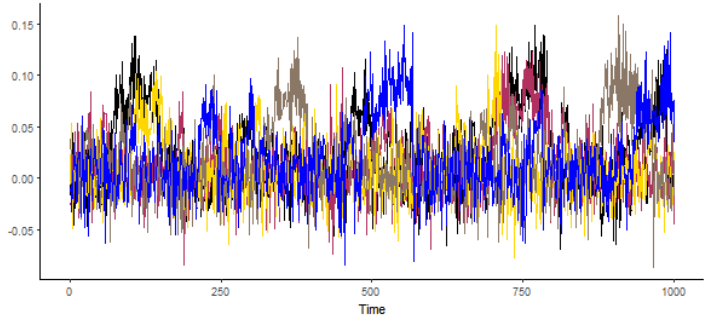
\includegraphics[scale=.42]{simplots2A}
	\label{fig:sim3plots}
\end{figure}
}

\frame{\frametitle{Chapter 1: LSTAR Model} 
\begin{figure}
	\centering
	\caption{Transition Function}
	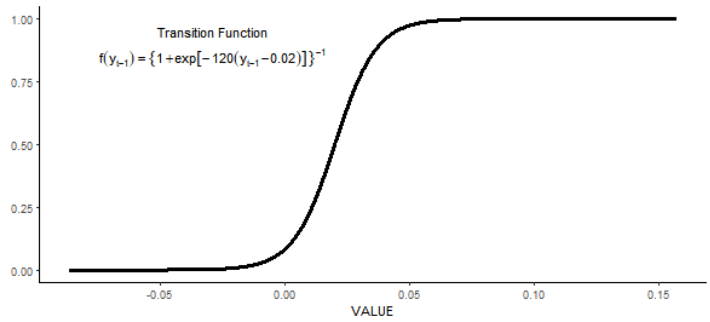
\includegraphics[scale=.42]{simplots2B}
	\label{fig:sim3plots}
\end{figure}
}

\frame{\frametitle{Chapter 1: LSTAR Model} 
\begin{figure}
	\centering
	\caption{Illustration of Regime-switching Behavior}
	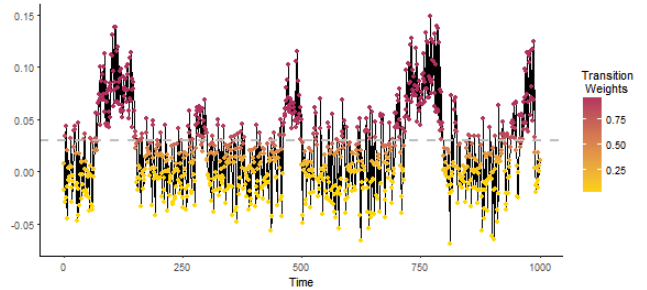
\includegraphics[scale=.5]{simplots2C}
	\label{fig:sim3plots}
\end{figure}
}

\frame{\frametitle{Chapter 1: LSTAR Model} 
\begin{itemize}
\item Bayesian Selection of the Threshold Variable (Scenario 1)\\~\

Consider Original Choice $z_{1,t}=y_{t-1}=[1,0,0,0]\bm{d}_t$. Posterior Means of $\bm{\phi}$ from 100 Replications are Plotted Below.
\begin{figure}[!h]
	\centering
      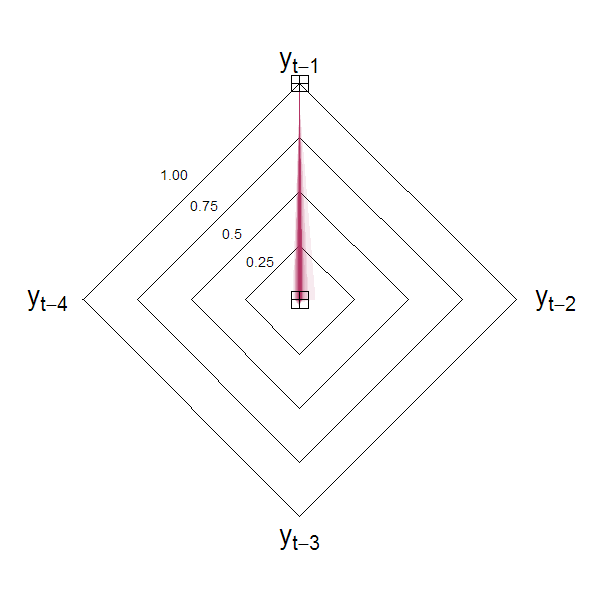
\includegraphics[scale=0.3]{hsthvar1}
\end{figure}
\end{itemize}
}

\frame{\frametitle{Chapter 1: LSTAR Model} 
\begin{itemize}
\item Bayesian Selection of the Threshold Variable (Scenario 2)\\~\

Consider  $z_{2,t}=y_{t-2}=[0,1,0,0]\bm{d}_t$. Posterior Means of $\bm{\phi}$ from 100 Replications are Plotted Below.
\begin{figure}[!h]
	\centering
      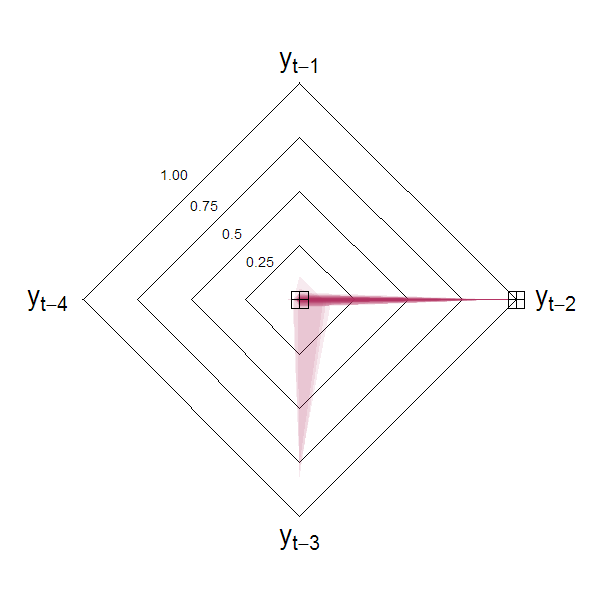
\includegraphics[scale=0.3]{hsthvar2}
\end{figure}
\end{itemize}
}

\frame{\frametitle{Chapter 1: LSTAR Model} 
\begin{itemize}
\item Bayesian Selection of the Threshold Variable (Scenario 3)\\~\

Consider  $z_{3,t}=\frac{y_{t-1}+y_{t-2}+y_{t-3}}{3}=[\frac{1}{3},\frac{1}{3},\frac{1}{3},0]\bm{d}_t$. Posterior Means of $\bm{\phi}$ from 100 Replications are Plotted Below.
\begin{figure}[!h]
	\centering
      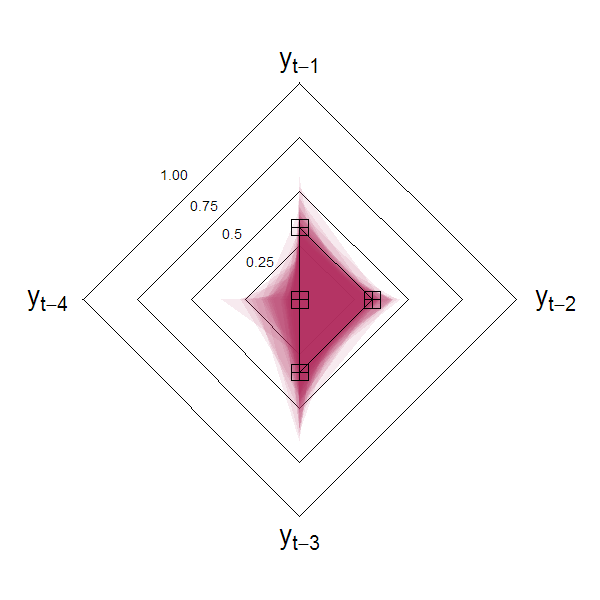
\includegraphics[scale=0.3]{hsthvar3}
\end{figure}
\end{itemize}
}

\frame{\frametitle{Chapter 1: LSTAR Model} 
\begin{itemize}
\item Application to Sunspot Data \citep{Granger1957,Terasvirta2010}\\~\
\item Application to Daily Maximum Water Temperatures \citep{Kamarianakis2016}\\~\
	\begin{itemize}
		\item Data Used From 31 Rivers in Spain
		\item Models to Forecast Daily Maximum Water Temperature
		\item Inclusion of Exogenous Distributed Lag Terms from Known Air Temperatures
		\item Horizon-Specific Models Targeting 3-step and 7-step Ahead Forecasts
		\item Nonlinear Models Improved Forecasting Accuracy for Some Rivers
	\end{itemize}
\end{itemize}
}

\frame{\frametitle{Chapter 1: LSTAR Model} 
\begin{itemize}
\item Contribution and Novelty \\~\
\begin{itemize}
	\item Efficacy of Bayesian Regularization for Nonlinear Time Series Models
	\item Use of the Dirichlet Prior Leads to More Encompassing LSTAR Specification
	\item Regime-Specific Tuning Parameters Influences Convergence in MCMC
	\item Detailed \textbf{R} Code Provided for Reproducibility \\~\
\end{itemize}
\item Feedback from \textit{International Journal of Forecasting} \\~\
\begin{itemize}
	\item Focus on Dirchlet Priors for Estimating Transition Variable
	\item Better Forecasting Application
	\item Consider Density Forecasts Along with Point Forecasts
\end{itemize}
\end{itemize}
}



%%%%%%%%%%%%%%%%%%%%%%%%%%%%%%%%%%%%%%%%%%%%%%%%%%%%%%%%%%%%%%%%%%%%%%%%
%% CHAPTER 2: THRESHOLD AUTOREGRESSIVE MODEL
%%%%%%%%%%%%%%%%%%%%%%%%%%%%%%%%%%%%%%%%%%%%%%%%%%%%%%%%%%%%%%%%%%%%%%%%
\frame{\frametitle{Chapter 2: TAR Model} 
\begin{itemize}
\item 
\end{itemize}

}








%%%%%%%%%%%%%%%%%%%%%%%%%%%%%%%%%%%%%%%%%%%%%%%%%%%%%%%%%%%%%%%%%%%%%%%%
%% CHAPTER 3: THRESHOLD AUTOREGRESSIVE MODEL
%%%%%%%%%%%%%%%%%%%%%%%%%%%%%%%%%%%%%%%%%%%%%%%%%%%%%%%%%%%%%%%%%%%%%%%%
\frame{\frametitle{Chapter 3: ARMA Model} 
\begin{itemize}
\item 
\end{itemize}

}








%%%%%%%%%%%%%%%%%%%%%%%%%%%%%%%%%%%%%%%%%%%%%%%%%%%%%%%%%%%%%%%%%%%%%%%%
%% FINISH: QUESTIONS
%%%%%%%%%%%%%%%%%%%%%%%%%%%%%%%%%%%%%%%%%%%%%%%%%%%%%%%%%%%%%%%%%%%%%%%%
\frame{\frametitle{} 
	\begin{center}
	\Huge Questions?
	\end{center}
}



























%%%%%%%%%%%%%%%%%%%%%%%%%%%%%%%%%%%%%%%%%%%%%%
\frame{\frametitle{Part 1: Bayesian Estimation of LSTAR Models}
\begin{itemize}
\item Primary Goals \\~\
	\begin{itemize}
		\item Establish the Efficacy of Bayesian Shrinkage Estimation applied to LSTAR
		\item Modify Bayesian Shrinkage Priors to Handle Regime-specific Sparsity
		\item Allow for Composite Transition Variable to Be Estimated Using Dirichlet Prior
	\end{itemize}
\end{itemize}
}

\frame{\frametitle{Part 1: Bayesian Estimation of LSTAR Models} 
\begin{itemize}
\item Bayesian Shrinkage Methods\\~\
\begin{itemize}
	\item Bayesian Lasso (BLASSO)
	\begin{equation*}
	\begin{split}
	\alpha_j|\sigma^2,\tau^2_{\alpha_j} \sim N(0,\sigma^2\tau^2_{\alpha_j}) \textrm{,  }  \tau^2_{\alpha_j}| \sim EXP(\lambda^2/2)\\ 
	 \beta_j|\sigma^2,\tau^2_{\beta_j}\sim N(0,\sigma^2\tau^2_{\beta_j}) \textrm{,  } \tau^2_{\beta_j}| \sim EXP(\lambda^2/2)
	\end{split}
\end{equation*}
	Hyperparameter $\lambda$ Controls Global Shrinkage Across Both Regimes. Following \cite{Park2008}, gamma hyperprior for $\lambda$ leads to inverse-Gaussian full conditional distribution.\\~\
	\item Regime-Specific Bayesian Lasso (RS-BLASSO) 
\begin{equation}
	 \tau^2_{\alpha_j}| \sim EXP(\lambda_1^2/2) \textrm{,  } \tau^2_{\beta_j}| \sim EXP(\lambda_2^2/2)
\end{equation}
Hyperparameters $\lambda_1$ and $\lambda_2$ control global shrinkage within low and high regimes, respectively.
\end{itemize}
\end{itemize}
}

\frame{\frametitle{Part 1: Bayesian Estimation of LSTAR Models} 
\begin{itemize}
\item Bayesian Shrinkage Methods (Cont.)\\~\
\begin{itemize}
	\item Variable Selection with Bayesian Lasso (VS-BLASSO) 
	Introducing latent binary variables $\zeta_j$ and $\eta_j$ for $j \in \{1,2,\cdots, p\}$, reparameterize $\alpha_j=\zeta_j\alpha_j^*$ and $\beta_j=\eta_j\beta_j^*$.
		\begin{equation*}
		\begin{split}
	 	\zeta_j \sim BERN(0.5) \textrm{,  } & \alpha_j^*|\sigma^2\sim DEXP\Big(0,\frac{\sigma^2}{\lambda}\Big) \\
	 	 \eta_j \sim BERN(0.5) \textrm{,  } & \beta_j^*|\sigma^2\sim DEXP\Big(0,\frac{\sigma^2}{\lambda}\Big)
		\end{split}
		\end{equation*}
	Method proposed by \cite{Lykou2011,Lykou2013}. Combines the subset selection approach of \cite{Kuo1998} with the Bayesian Lasso of  \cite{Park2008}.
\end{itemize}
\end{itemize}
}

\frame{\frametitle{Part 1: Bayesian Estimation of LSTAR Models} 
\begin{itemize}
\item Bayesian Shrinkage Methods (Cont.)\\~\
\begin{itemize}
	\item Bayesian Horseshoe (BHS)
	\begin{equation*}
	\begin{split}
	\alpha_j|\lambda_{\alpha_j} & \sim N(0,\lambda_{\alpha_j}) \textrm{,  }  \beta_j|\lambda_{\beta_j} \sim N(0,\lambda_{\beta_j}) \\
	  \lambda_{\alpha_j} & \sim C^+(0,\lambda) \textrm{,  } \lambda_{\beta_j} \sim C^+(0,\lambda) \\
	  \lambda|\sigma^2 & \sim C^+(0,\sigma)
	\end{split}
	\end{equation*}
	Although hyperparameter $\lambda$ provides global shrinkage, the additional  hyperparameters allow for finer shrinkage locally.
\end{itemize}
\end{itemize}
}




















%%%%%%%%%%%%%%%%%%%%%%%%%%%%%%%%%%%%%%%%%%%%%%
\frame{\frametitle{Part 2: Bayesian Estimation of TAR Models}
\begin{itemize}
\item Primary Goals\\~\
\begin{itemize}
\item Explore Modeling Approaches for Traffic Occupancy Using Autoregressive Distributed Lag (ARDL) Models and Threshold Autoregressive Distributed Lag (TARDL) Models.
\item Combine Bayesian Shrinkage with Projection Predictive Variable Selection to Obtain Sparse Estimation Focused on Optimal Forecasting \citep{Piironen2017}
\item Modify Above Methodology to Handle Regime-Specific Sparsity Patterns
\item Evaluate Models on Short-Term Forecasting at Multiple Horizons
\end{itemize}
\end{itemize}
}

\frame{\frametitle{Part 2: Bayesian Estimation of TAR Models} 
\begin{itemize}
\item Modeling Traffic Occupancy \\~\
	\begin{itemize}
		\item Advanced Traffic Management Systems (ATMS) Monitor Traffic Characteristics in Real Time
		\item ATMS Require Fast Short-Term Forecasting to Reduce Congestion
		\item Most Modeling Approaches Aimed at Traffic Flow and Speed \citep{Smith1997, Vlahogianni2014}
		\item Different Regimes of Traffic: Free-Flow, Congested, Transitional
		\item Factors Influencing Regime Changes : Weekly Work Patterns, Accidents, Weather, etc.
		\item Traffic Occupancy is the Percent of Time a Detection Zone is Occupied
		\item Capture Spatio-Temporal Dependencies with ARDL and TARDL Models
	\end{itemize}
\end{itemize}
}

\frame{\frametitle{Part 2: Bayesian Estimation of TAR Models} 
\begin{itemize}
\item Traffic Data Used \\~\
	\begin{itemize}
		\item Major Athens' Arterial: Alexandras Ave.
		\item Traffic Occupancy Measured on 90s Interval
		\item Time Period: April 2000
		\item Obtained by National Technical University of Athens
		\item Provided for 2013 TRANSportation Data FORecasting Competition (TRANSFOR) Developed by the Traffic Research Board (TRB) for Annual Meeting Workshop \citep{Kamarianakis2012}
		\item Mean Aggregate to 3-min Interval for Moderate Smoothing
	\end{itemize}
\end{itemize}
}

\frame{\frametitle{Part 2: Bayesian Estimation of TAR Models} 
\begin{itemize}
\item Traffic Data Used (Cont.) \\~\

Focus on Data From 3 Loop Detectors Identified as $A$, $B$, and $C$ Along Westbound Direction. Illustrated from Google Maps.
\begin{figure}[!h]
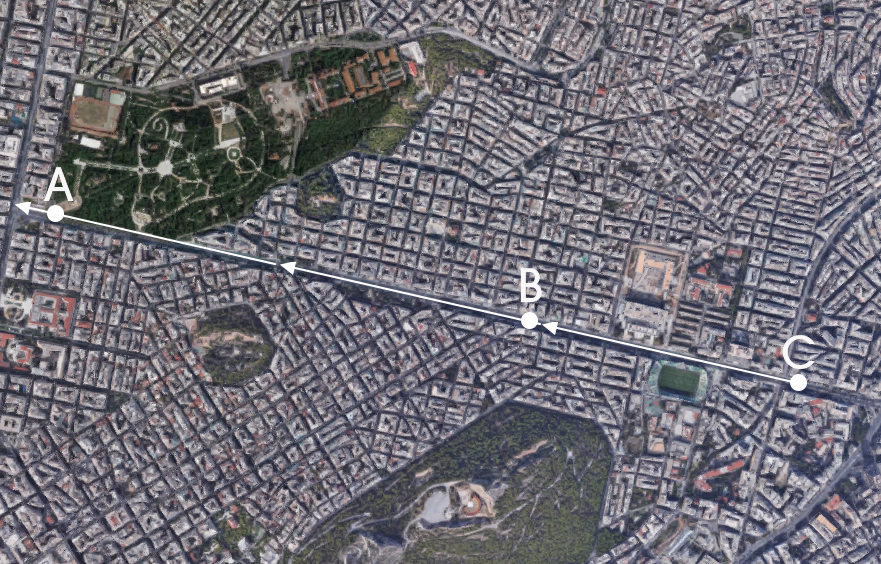
\includegraphics[scale=0.25]{TrafficMap}
\end{figure}
\end{itemize}
}

\frame{\frametitle{Part 2: Bayesian Estimation of TAR Models} 
\begin{itemize}
\item Primary Focus \\~\

Let  $O_{L,t}=$ Traffic occupancy for location $L \in\{A,B,C\}$ at time $t$ \\~\

For each day $D\in\{M,T,W,Th,F\}$ and  horizon $h \in \{1,3,5\}$, we develop and compare $(D,h)$-specific models for $O_{B,t}$. \\~\

Since $O_{L,t} \in [0,1]$, models are built using $Y_{L,t}=\log[O_{L,t}/(1-O_{L,t})]$ \citep{Wallis1987}. \\~\

Models designed to ``directly'' forecast $Y_{B,t+h}$ given previously known information $\mathcal{I}=\{Y_{A,k},Y_{B,k},Y_{C,k}| k \leq t\}$

\end{itemize}
}

\frame{\frametitle{Part 2: Bayesian Estimation of TAR Models} 
\begin{itemize}
\item  Primary Focus (Cont.) \\~\
Time Series Plots of $O_{A,t}$ (\textit{maroon}), $O_{B,t}$ (\textit{black}), and $O_{C,t}$ (\textit{blue})
\begin{figure}[!h]
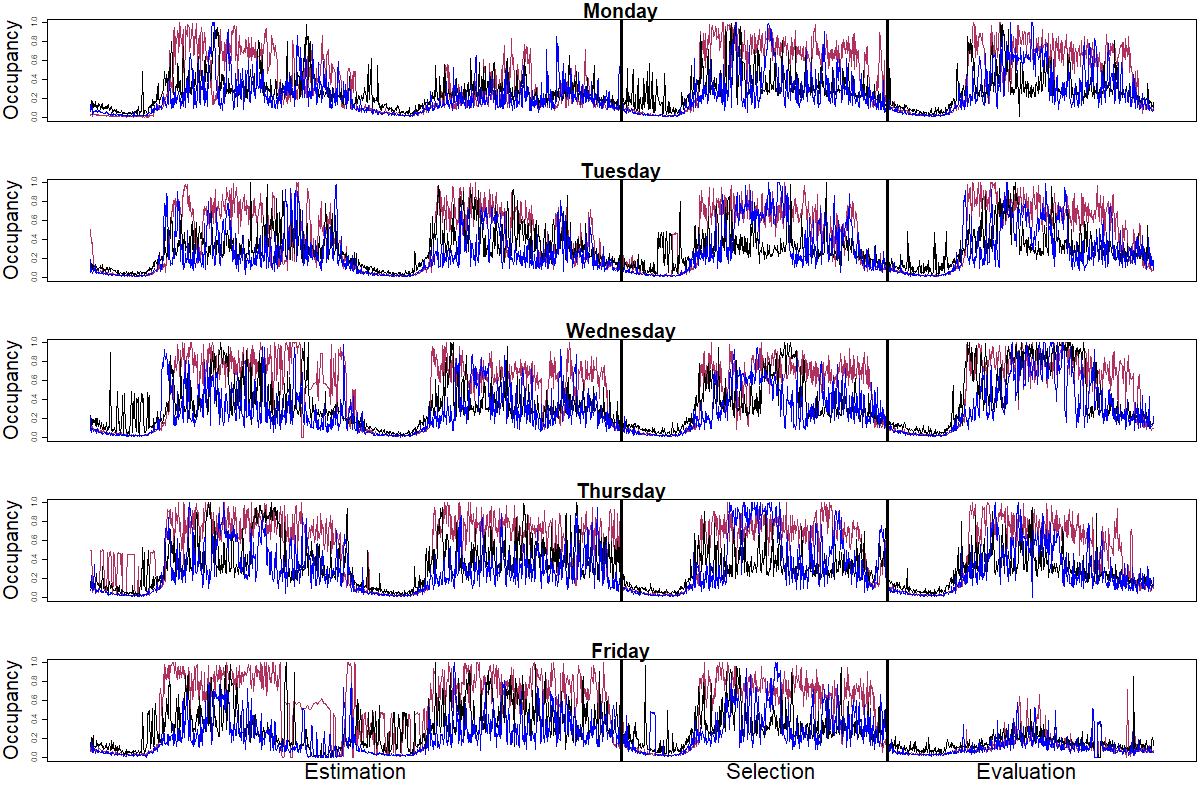
\includegraphics[scale=0.23]{OrigPlotTrafficOcc}
\end{figure}
\end{itemize}
}












\frame{\frametitle{Part 2: Bayesian Estimation of TAR Models} 
\begin{itemize}
\item Baseline Models
\begin{itemize}
	\item Horizon Specific Random Walks  $\mathcal{W}(D,h)$
	\begin{equation*}	
		Y_{B,t}=Y_{B,t-h}+\epsilon_t
	\end{equation*}
	\item Harmonic Seasonal Profile $\mathcal{S}_L(D)$\\~\
	
	Build Daily Seasonal Profiles for All Locations of Interest. These Models Can Be Used to Forecast at All Horizons
	\begin{equation*}
		Y_{L,t}=\mu_{L,t}+\sum\limits_{t=1}^{S} \Big[\alpha_{L,t}\sin\Big(\frac{2\pi t}{480}\Big)+\beta_{L,t}\cos\Big(\frac{2\pi t}{480}\Big)\Big]+		\epsilon_{L,t}
	\end{equation*}
\end{itemize}
\end{itemize}
}

\frame{\frametitle{Part 2: Bayesian Estimation of TAR Models} 
\begin{itemize}
\item Models Using Raw Traffic Occupancies\\~\

Define $\bm{Y_{L,t-h}}'=[Y_{L,t-h},Y_{L,t-h-1},\cdots,Y_{L,t-h-P+1}]$
\begin{itemize}
	\item ARDL $\mathcal{L}_1(D,h)$
	\begin{equation*}
		Y_{B,t}=\mu+\bm{\alpha}'\bm{Y_{A,t-h}}+\bm{\beta}'\bm{Y_{B,t-h}}+\bm{\gamma}'\bm{Y_{C,t-h}}+\epsilon_t
	\end{equation*}
	\item TARDL $\mathcal{R}_1(D,h)$\\~\
	\begin{equation*}
Y_{B,t}=
  \begin{cases}
    \mu_L+\bm{\alpha_L}'\bm{Y_{A,t-h}}+\bm{\beta_L}'\bm{Y_{B,t-h}}+\bm{\gamma_L}'\bm{Y_{C,t-h}}+\epsilon_{t,L} & \textrm{ if } Y_{B,t-h}<\delta \\
    \mu_H+\bm{\alpha_H}'\bm{Y_{A,t-h}}+\bm{\beta_H}'\bm{Y_{B,t-h}}+\bm{\gamma_H}'\bm{Y_{C,t-h}}+\epsilon_{t,H} & \textrm{ if } Y_{B,t-h}>\delta \\
  \end{cases}
\end{equation*}
\end{itemize}
\end{itemize}
}

\frame{\frametitle{Part 2: Bayesian Estimation of TAR Models} 
\begin{itemize}
\item Models Using Deviations From Seasonal Profiles \\~\

Define $\Delta_{L,t}=Y_{L,t}-\widehat{Y}_{L,t}$ as the deviation from the seasonal profile for location $L$ at time $t$. 

Also, define $\bm{\Delta_{L,t-h}}'=[\Delta_{L,t-h},\Delta_{L,t-h-1},\cdots,\Delta_{L,t-h-P+1}]$.


\begin{itemize}
	\item ARDL $\mathcal{L}_2(D,h)$
\begin{equation*}
\Delta_{B,t}=\mu+\bm{\alpha}'\bm{\Delta_{A,t-h}}+\bm{\beta}'\bm{\Delta_{B,t-h}}+\bm{\gamma}'\bm{\Delta_{C,t-h}}+\epsilon_t
\end{equation*}
	\item TARDL $\mathcal{R}_2(D,h)$\\~\
\begin{equation*}
\Delta_{B,t}=
  \begin{cases}
    \mu_L+\bm{\alpha_L}'\bm{\Delta_{A,t-h}}+\bm{\beta_L}'\bm{\Delta_{B,t-h}}+\bm{\gamma_L}'\bm{\Delta_{C,t-h}}+\epsilon_{t,L} & \textrm{ if } Y_{B,t-h}<\delta \\
    \mu_H+\bm{\alpha_H}'\bm{\Delta_{A,t-h}}+\bm{\beta_H}'\bm{\Delta_{B,t-h}}+\bm{\gamma_H}'\bm{\Delta_{C,t-h}}+\epsilon_{t,H} & \textrm{ if } Y_{B,t-h}>\delta \\
  \end{cases}
\end{equation*}
\end{itemize}
\end{itemize}
}

\frame{\frametitle{Part 2: Bayesian Estimation of TAR Models} 
\begin{itemize}
	\item Model Complexity\\~\
	
	Consider Full Model  $\mathcal{M} \in \{L_1(D,h),R_1(D,h),L_2(D,h),R_2(D,h)\}$.
	Define Parameter Vector $\bm{\theta}_{\mathcal{M}}\in \bm{\Theta}_\mathcal{M}$. The dimensionality $\dim(\bm{\Theta}_\mathcal{M})$ increases with with $S$ and  $P$.
	\begin{table}[!h]
  \footnotesize
  \centering
    \begin{tabular}{cc}
    \toprule
   Model & $\dim(\bm{\Theta})$  \\
    \midrule
    $\mathcal{W}(D,h)$ & $1$ \\
    $\mathcal{S}_B(D)$ & $2S+2$ \\
    $\mathcal{L}_1(D,h)$ & $3P+1+1=3P+2$ \\
    $\mathcal{R}_1(D,h)$ & $2(3P+2)=6P+4$ \\
    $\mathcal{L}_2(D,h)$ & $3(2S+2)+ 3P+2=6S+3P+8$ \\
    $\mathcal{R}_2(D,h)$ & $3(2S+2)+6P+4=6S+6P+10$ \\
    \bottomrule
    \end{tabular}%
\end{table}%
\end{itemize}
}

\frame{\frametitle{Part 2: Bayesian Estimation of TAR Models} 
\begin{itemize}
	\item Consider General TAR($P$) Model
	
	\begin{equation*}
\begin{split}
y_t&=
  \begin{cases}
    \alpha_0+\alpha_1y_{t-1}+\alpha_2y_{t-2}+\cdots+\alpha_Py_{t-P}+\epsilon_{\alpha,t} & \textrm{ if } z_t<\delta \\
    \beta_0+\beta_1y_{t-1}+\beta_2y_{t-2}+\cdots+\beta_Py_{t-P}+\epsilon_{\beta,t} & \textrm{ if } z_t>\delta \\
  \end{cases}\\
  &=
    \begin{cases}
    \bm{\alpha}'\bm{y_{t-1}} +\epsilon_{\alpha,t} & \textrm{ if } z_t<\delta \\
     \bm{\beta}'\bm{y_{t-1}} +\epsilon_{\beta,t} & \textrm{ if } z_t>\delta \\
  \end{cases}\\
  \textrm{ where } & \epsilon_{\alpha,t} \sim N(0,\sigma^2_\alpha) \textrm{ and } \epsilon_{\beta,t} \sim N(0,\sigma^2_\beta)
  \end{split}
\end{equation*}
	
	For future reference, we abbreviate the full TAR($P$) model $\mathcal{M}_R$. \\~\
	
	Model $\mathcal{M}_R$ is fully defined by parameter vector $\bm{\theta}_{\mathcal{M}_R}'=[\bm{\alpha}',\bm{\beta}',\sigma_\alpha,\sigma_\beta,\delta]$. \\~\
	
	Furthermore, let $\mathcal{M}_{LR}$ and $\mathcal{M}_{HR}$ represent the low-regime and high-regime models, respectively.\\~\
	

From the $2^{2(P+1)}$ submodels, we aim to identify the best submodel $\mathcal{M}^*_R$
\end{itemize}
}

\frame{\frametitle{Part 2: Bayesian Estimation of TAR Models} 
\begin{itemize}
\item Methodology Step 1: Bayesian Shrinkage\\~\

Apply Regime-Specific BHS for Initial Sparse Estimation
\begin{equation*}
\label{eq:hsp}
\begin{split}
 	\alpha_j &\sim N(0,\sigma^2_\alpha\lambda^2_{\alpha_j}\lambda_{\alpha}^2), \textrm{ } \lambda_{\alpha_j}\sim C^+(0,1), \textrm{ } \lambda_\alpha \sim C^+(0,1) \\
 	\beta_j & \sim N(0,\sigma^2_\beta\lambda^2_{\beta_j}\lambda_{\beta}^2), \textrm{ } \lambda_{\beta_j}\sim C^+(0,1), \textrm{ } \lambda_\beta \sim C^+(0,1)\\
 	& \forall j \in \{1,2,3,\cdots,P\}
\end{split}
\end{equation*}

\end{itemize}
}

\frame{\frametitle{Part 2: Bayesian Estimation of TAR Models} 
\begin{itemize}
	\item Methodology Step 2: Projection Predictive Variable Selection\\~\
	\begin{itemize}
		\item Kullback-Leibler (KL) Divergence
		\begin{itemize}
			\item Asymmetric Measure of Distance Between 2 Probability Distributions
			\item Developed by \cite{Goutis1998, Dupuis2003,Piironen2017} for Generalized Linear Models
			\item Measure Discrepancy Between Full Model $\mathcal{M}_R$ and Proposed Submodel $\mathcal{M}^\perp_R$ \\~\
		\end{itemize}
		\item Necessary Definitions
			$$\textrm{Matrix } \bm{Y_{t-1}} \textrm{ where $k$th row is } \bm{y_{k-1}}'=[1,y_{k-1},y_{k-2},\cdots,y_{k-P}]$$
			$$\textrm{Regime-Specific Full Reference Models: } \mathcal{M}_{LR} \textrm{ and } \mathcal{M}_{HR}$$
			$$\textrm{Regime-Specific Submodels: } \mathcal{M}^\perp_{LR} \textrm{ and } \mathcal{M}^\perp_{HR}$$
	\end{itemize}
\end{itemize}
}

\frame{\frametitle{Part 2: Bayesian Estimation of TAR Models} 
\begin{itemize}
	\item Methodology Step 2: Projection Predictive Variable Selection (Cont.)\\~\
	 \begin{itemize}
		\item Regime-Specific Projection Approach\\~\
		\begin{equation*}
		\begin{split}
		f(\bm{\theta}_{\mathcal{M}_R}|\mathcal{M}_R,Data) & \to f(\bm{\theta}_{\mathcal{M}^\perp_R}|\mathcal{M}^\perp_R,Data)\\
		\bm{\theta}^{(s)} & \to \bm{\theta}^{\perp(s)}\\
		[\bm{\alpha}^{(s)},\sigma_\alpha^{(s)},\bm{\beta}^{},\sigma_\beta^{(s)},\delta^{(s)}] & \to [\bm{\alpha}^{\perp(s)},\sigma_\alpha^{\perp(s)},\bm{\beta}^{\perp(s)},\sigma_\beta^{\perp(s)},\delta^{(s)}]\\
		\end{split}
		\end{equation*}
		\item Regime-Specific Projection Process

\indent Split $\bm{Y_{t-1}}$ into $\bm{Y_{LR,t-1}}$ and $\bm{Y_{HR,t-1}}$ based on $\delta^{(s)}$.

\indent Identify $\bm{Y^\perp_{LR,t-1}}$ and $\bm{Y^\perp_{HR,t-1}}$ based on proposed  $\mathcal{M}^\perp_{LR}$ and $\mathcal{M}^\perp_{HR}$

\begin{equation*}
\scriptsize
\begin{split}
\bm{\alpha}^{\perp(s)}&=(\bm{Y^{\perp'}_{LR,t-1}}\bm{Y^{\perp}_{LR,t-1}})^{-1} \bm{Y^{\perp'}_{LR,t-1}}     \bm{Y_{LR,t-1}}\bm{\alpha}^{(s)}\\
\sigma_\alpha^{\perp(s)}&=\sqrt{\sigma_\alpha^{(s)}+\frac{( \bm{Y_{LR,t-1}}\bm{\alpha}^{(s)}-\bm{Y^\perp_{LR,t-1}}\bm{\alpha}^{\perp(s)})'( \bm{Y_{LR,t-1}}\bm{\alpha}^{(s)}-\bm{Y^\perp_{LR,t-1}}\bm{\alpha}^{\perp(s)})}{T}                                  }\\
\bm{\beta}^{\perp(s)}&=(\bm{Y^{\perp'}_{HR,t-1}}\bm{Y^{\perp}_{HR,t-1}})^{-1} \bm{Y^{\perp'}_{HR,t-1}} \bm{Y_{HR,t-1}}\bm{\beta}^{(s)}\\
\sigma_\beta^{\perp(s)}&=\sqrt{\sigma_\beta^{(s)}+\frac{( \bm{Y_{HR,t-1}}\bm{\beta}^{(s)}-\bm{Y^\perp_{HR,t-1}}\bm{\beta}^{\perp(s)})'( \bm{Y_{HR,t-1}}\bm{\beta}^{(s)}-\bm{Y^\perp_{HR,t-1}}\bm{\beta}^{\perp(s)})}{T}                                   }
\end{split}
\end{equation*}
	\end{itemize}
\end{itemize}
}

\frame{\frametitle{Part 2: Bayesian Estimation of TAR Models} 
\begin{itemize}
	\item Methodology Step 2: Projection Predictive Variable Selection (Cont.)\\~\
	 \begin{itemize}
		\item Regime-Specific Projection Process (Cont.)\\~\
		For each $\bm{\theta}^{(s)}$, we obtain regime-specific KL divergences,
\begin{equation*}
\begin{split}
d^{(s)}_{LR}(\bm{\alpha}^{(s)},\sigma^{(s)}_\alpha)&=\frac{1}{2}\log\bigg(\frac{\sigma^{\perp(s)}_\alpha}{\sigma^{(s)}_\alpha}\bigg)\\
d^{(s)}_{HR}(\bm{\beta}^{(s)},\sigma^{(s)}_\beta)&=\frac{1}{2}\log\bigg(\frac{\sigma^{\perp(s)}_\beta}{\sigma^{(s)}_\beta}\bigg)
\end{split}
\end{equation*}
	
		Finally, we measure regime-specific discrepancies by
\begin{equation*}
\begin{split}
D(\mathcal{M}_{LR}||\mathcal{M}^\perp_{LR})&=\frac{1}{S}\sum\limits^S_{s=1} d^{(s)}_{LR}(\bm{\alpha}^{(s)},\sigma^{(s)}_\alpha)    \\
D(\mathcal{M}_{HR}||\mathcal{M}^\perp_{HR})&=\frac{1}{S}\sum\limits^S_{s=1} d^{(s)}_{HR}(\bm{\beta}^{(s)},\sigma^{(s)}_\beta)     \\
\end{split}
\end{equation*}
	\end{itemize}
\end{itemize}
}

\frame{\frametitle{Part 2: Bayesian Estimation of TAR Models} 
\begin{itemize}
	\item Methodology Step 2: Projection Predictive Variable Selection (Cont.)\\~\
	 \begin{itemize}
		\item Forward Stepwise Selection Algorithm\\~\
		
		For Intercept-only Models $\mathcal{M}^0_{LR}$ and $\mathcal{M}^0_{HR}$, calculate initial discrepancies $D(\mathcal{M}_{LR}||\mathcal{M}^0_{LR})$ and $D(\mathcal{M}_{HR}||\mathcal{M}^0_{HR})$	\\~\
	
		For each level of flexibility $p \in \{1,2,\cdots,P\}$, we identify the best regime-specific submodels $\mathcal{M}^p_{LR}$ and $\mathcal{M}^p_{HR}$.\\~\
		
		Algorithm conducted such that for $j<k$ $\mathcal{M}^j_{HR}$ is nested in $\mathcal{M}^k_{HR}$.
	\end{itemize}
\end{itemize}
}

\frame{\frametitle{Part 2: Bayesian Estimation of TAR Models} 
\begin{itemize}
	\item Methodology Step 3: Final Model Selection\\~\
	 \begin{itemize}
		\item Choose $\mathcal{M}^*_{LR}$ and $\mathcal{M}^*_{HR}$ Based on Relative Explanatory Power \\~\
		\begin{equation*}
\begin{split}
RelE(\mathcal{M}^p)&=1-\frac{D(\mathcal{M}||\mathcal{M}^p)}{D(\mathcal{M}||\mathcal{M}^0)}\\
\end{split}
\end{equation*}
		\item Choose Based On Minimization of RMSFE for Time Period Intentionally Ignored
		\begin{equation*}
  			RMSFE(\mathcal{M}^p)=\sqrt{\frac{1}{T}\sum (y_t-\hat{y}_t)^2}
		\end{equation*}
	\end{itemize}
\end{itemize}
}

















%%%%%%%%%%%%%%%%%%%%%%%%%%%%%%%%%%%%%%%%%%%%%%5
\frame{\frametitle{Part 3: Current Status and Future Directions} 
\begin{itemize}
\item Bayesian Shrinkage Estimation of Logistic Smooth Transition Autoregressions \\~\
	\begin{itemize}
		\item Submitted to \textit{Communications in Statistics: Simulation and Compuation} on June 19, 2017
		\item Code Implementing Bayesian Shrinkage Estimation for Coefficients and Dirichlet Prior for Composite Threshold Variable was Included in Paper Submission
		\item Decision has not been Made \\~\
	\end{itemize}
	\item Sparse Bayesian Linear and Nonlinear Models Estimated for Short-Term Forecasting of Traffic Occupancy \\~\
	\begin{itemize}
		\item Plan to Submit to \textit{International Journal of Forecasting} Before December
		\item Code Applying Horseshoe Priors and Projection Approach to AR and TAR Models Will Be Included in Submission
	\end{itemize}
\end{itemize}
}

\frame{\frametitle{Part 3: Current Status and Future Directions} 
\begin{itemize}
\item Additions to Second Paper \\~\
	\begin{itemize}
		\item Model Traffic Occupancy for Loop Detectors in Eastbound Direction
		\item Build and Evaluate a Combined Model Analogous to Error Correction Models
		\item Compare to Models Intentionally Ignoring Information from Nearby Locations
		\item Incorporate Traffic Volume and Speed in Models for Traffic Occupancy
	\end{itemize}
\end{itemize}
}

\frame{\frametitle{Part 3: Current Status and Future Directions} 
\begin{itemize}
\item Future Research Ideas \\~\
	\begin{itemize}
		\item Bayesian Shrinkage and Selection Ideas to Generalized Nonlinear Models.
		\item Model Traffic Occupancy Using Linear and Nonlinear Beta AR Models
		 	$$O_t \sim Beta(\mu_t\phi_t,\mu_t(1-\phi_t))$$
		 	$$log\bigg(\frac{\mu_t}{1-\mu_t}\bigg)=f_1(y_{t-1},y_{t-2},\cdots,y_{t-P})$$
		 	$$log(\phi)=f_2(y_{t-1},y_{t-2},\cdots,y_{t-P})$$
	\end{itemize}
\end{itemize}
}

\frame{\frametitle{Part 3: Current Status and Future Directions} 
\begin{itemize}
\item Future Research Ideas (Cont.) \\~\
	\begin{itemize}
		\item Bayesian Regularization and Multicollinearity. Naturally occurs in AR, LSTAR, TAR, ARDL, and TARDL Models. \\~\
		
		 For  $T \in \{50,100,200\}$, $\phi_1 \in \{0.9,0.7,0.5\}$ and  $\phi_2 \in \{-0.9,-0.7,-0.5\}$, we generate 100 replications of length $T$ under the below specifications:
		$$x_{1,t}=\phi_1 x_{1,t-1}+\epsilon_{1,t} \textrm{ and } x_{2,t}=\phi_2 x_{2,t-1}+\epsilon_{2,t}$$
		$$y_t=80+8x_{1,t-1}-6x_{1,t-3}-8x_{2,t-2}+6x_{2,t-4}+\epsilon_t$$
	For $P \in \{5,10,20\}$, we compare shrinkage methods on parameter estimation and variable selection errors. \\~\
		\item Bayesian Approaches to Forecast Combinations from Naive, Linear, and Nonlinear Models.
		\begin{itemize}
			\item Consider Static and Dynamic Approaches to Weighting Schemes.
			\item Possible Value in Nonlinear Combination Schemes
		\end{itemize}
	\end{itemize}
\end{itemize}
}






























\frame[allowframebreaks]{\frametitle{References}
    {\footnotesize
    \bibliographystyle{apalike}
    \bibliography{phd}
    }
}

\end{document}

